\chapter{Implementation}

\section{System Architecture}
\label{sec:sys-arch}

\begin{figure}[ht]
    \centering
    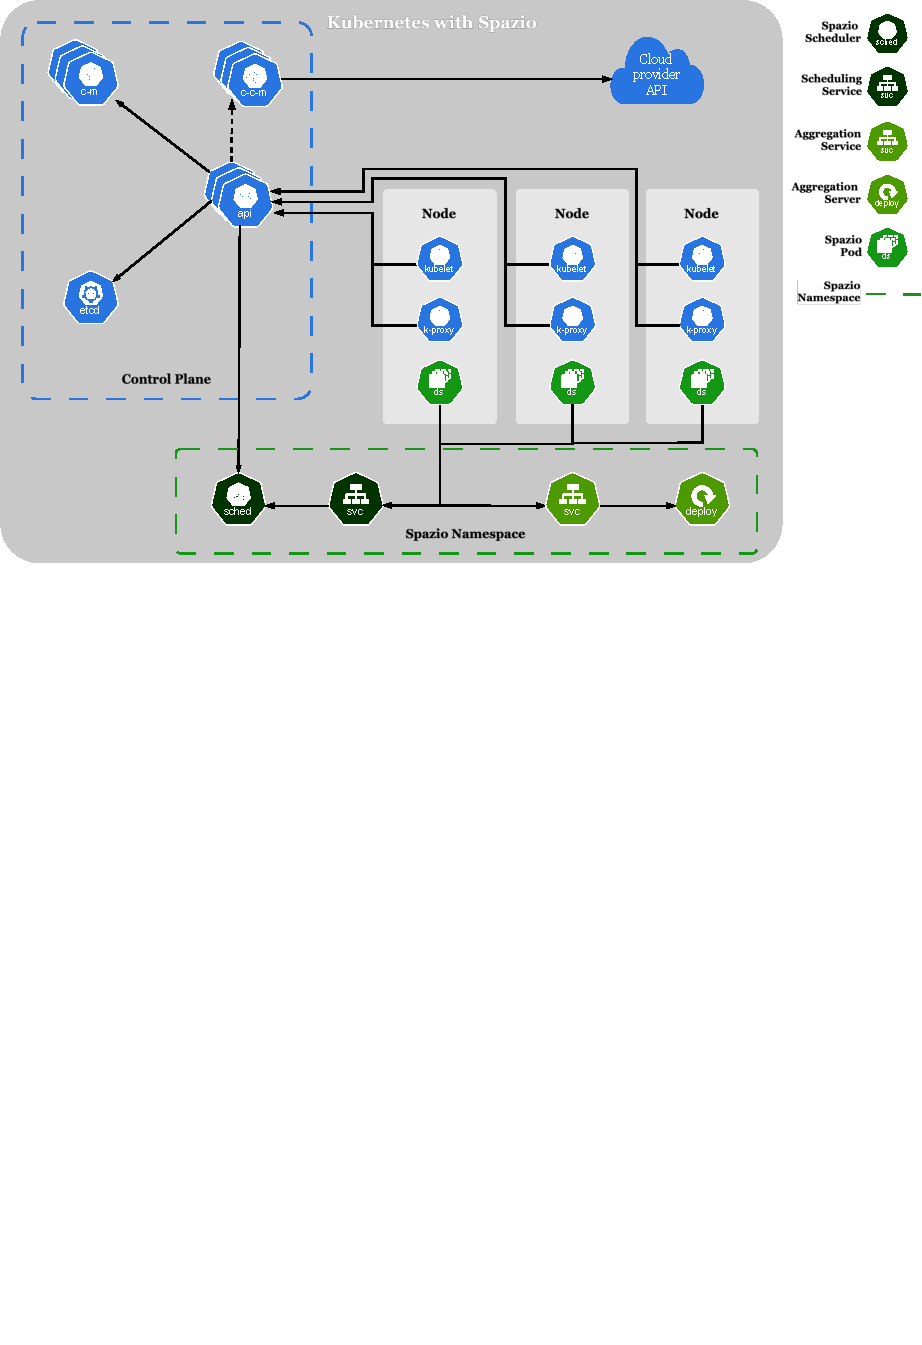
\includegraphics[width=\textwidth]{images/carico-svg.pdf}
    \caption{The components within the \textsc{Carico} system}
    \label{fig:spazio-system}
\end{figure}

The \textsc{Carico} system consists of three core components (Figure
\ref{fig:spazio-system}):
\begin{itemize}
    \item \textsc{Carico} DaemonSet: This Pod collectes telemetry from a
        Node and generates its subspace and Pod-Capacity  signal. This signal is
        periodically sent to the Scheduling Service. When the \textsc{Carico}
        Pod deems its subspace outdated, it requests the latest aggregated
        subspace from the Aggregation service.
    \item Aggregation Server: This Pod performs Subspace-Merge on incoming
        subspaces, and returns the latest aggregated subspace.
    \item Scheduler: The scheduler filters and scores Nodes based on their
        latest Pod-Capacity.
\end{itemize}

\section{\textsc{Carico} Pod}
\begin{figure}[H]
    \centering
    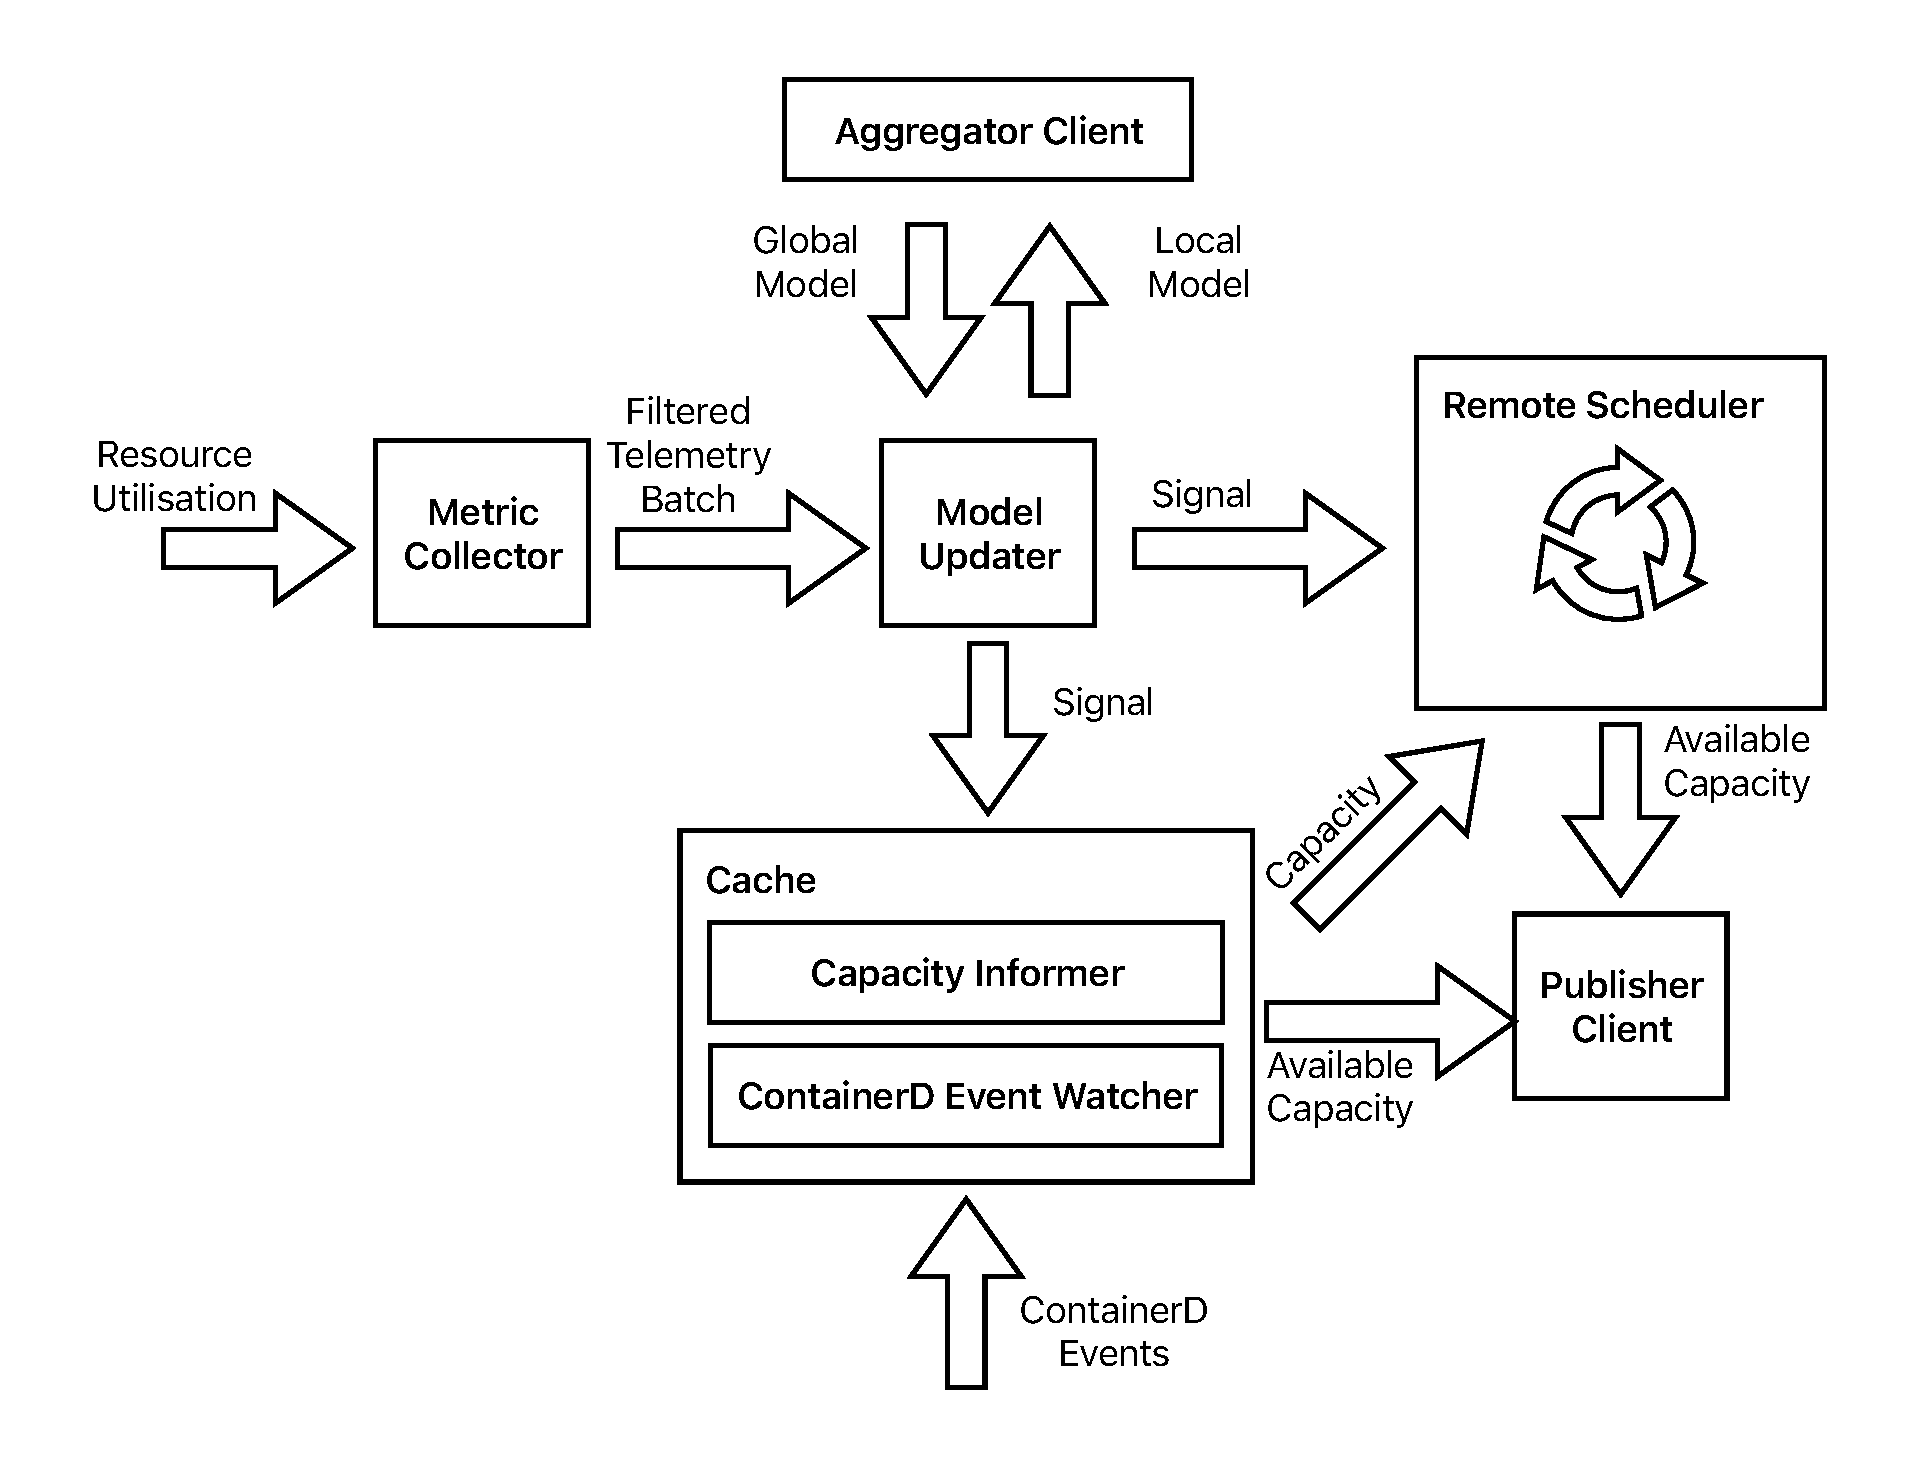
\includegraphics[width=\textwidth]{images/spazio-pod.pdf}
    \caption{Core components within the \textsc{Carico} Pod}
    \label{spazio-pod-components}
\end{figure}
The goal of \textsc{Carico} Pods is to accurately generate its Node's
Pod-Capacity. This necessitates high quality telemetry for subspace creation and
effective signal processing techniques to estimate Baseline and Per-Pod-Cost.
Kubernetes dynamically changing workloads also required \textsc{Carico} Pods to
frequently update its subspace and Pod-Capacity signal. However, updating too
frequently could result in large overheads and reduce the available resources.
Investigations using the prototype showed that an update frequency of 1Hz
achieved the best results.

\subsection{Metric Collection}
To achieve an update frequency of 1Hz, \textsc{Carico} Pods must collect batches
of telemetry data every second. To construct a batch of telemetry,
\textsc{Carico} Pods must periodically poll resource metrics and [0,1]-normalise
them. This polling frequency is also limited by the overhead it incurrs. I
explored two primary sources of telemetry data:
\begin{itemize}
    \item Metrics Server: a cluster add-on that acts as a centralised source of
        container reosurce metrics.
    \item \verb|/proc/|: a pseudo-filesystem within Linux that exposes real-time
        information about running processes and system's hardware.
\end{itemize}

Metrics Server uses a scraper to periodically (default every 15 seconds) collect
resource metrics from Kubelets and exposes them from its
\verb|metrics.k8s.io/v1| APIService. While simple to use, it offers limited
metrics (CPU and RAM utilisation only) and introduces additional latency.
Moreover, its default scraping interval is too infrequent, potentially missing
short-lived Pods entirely.

\verb|/proc/|, conversely, offers low latency access to an up-to-date view
of the current state of the system. Furthermore, \verb|/proc/| contains various
files and subdirectories, each providing specific information about different
types of resources. Furthermore, these sources are not generated periodically,
but rather on-the-fly. This guarantees that the information you see is as
current as the system's internal state and allows for polling of resource
metrics at higher frequencies. \textsc{Carico} Pods use a polling
frequency of 10Hz, providing enough samples to accurately construct the subspace
(10 samples) without incurring too large of an overhead.

The next challenge was to select resource metrics, with which to build the
subspace, that could be [0,1]-normalised to indicate full or no capacity. The
subsequent subsections detail the resource metrics I considered and the
rationale behind their use.
% I decided to collect CPU and memory utilisation as my telemetry data, as these
% metrics are easily accessible and are used in a variety of industry-standard
% schedulers
 % In addition, it would take $15 \times \text{batch size}$
% seconds between model updates (required to collect a single
% batch before performing subspace merging), and would result in a less
% representative and out-of-date model of "current" resource usage.

\subsubsection{Utilisation Metrics}
Standard utilisation metrics (e.g., CPU and memory percentage usage) are widely
used in industry~\cite{hadoop2016apache,sahasrabudhe_improved_2015}.

\texttt|/proc/stat| file reports the cumulative count of "jiffies" (typically
hundredths of a second) each CPU spent in a specific mode \cite{proc_stat5}. The
[0,1]-normalised CPU utilisation can then be calculated using:
\[ \text{CPU Usage\%} = 1 - \frac{\Delta\text{idle} +
\Delta\text{iowait}}{\Delta\text{across all fields}} \]
In addition, \verb|/proc/meminfo| shows a snapshot of the memory usage in
kilobytes. The [0,1]-normalised memory usage can then be calculated from the given
field:
\[ \text{Memory Used\%} = 1 - \frac{\text{MemFree} +
\text{Buffers} + \text{Cached}}{\text{MemTotal}}\]

\begin{figure}[H]
    \centering
    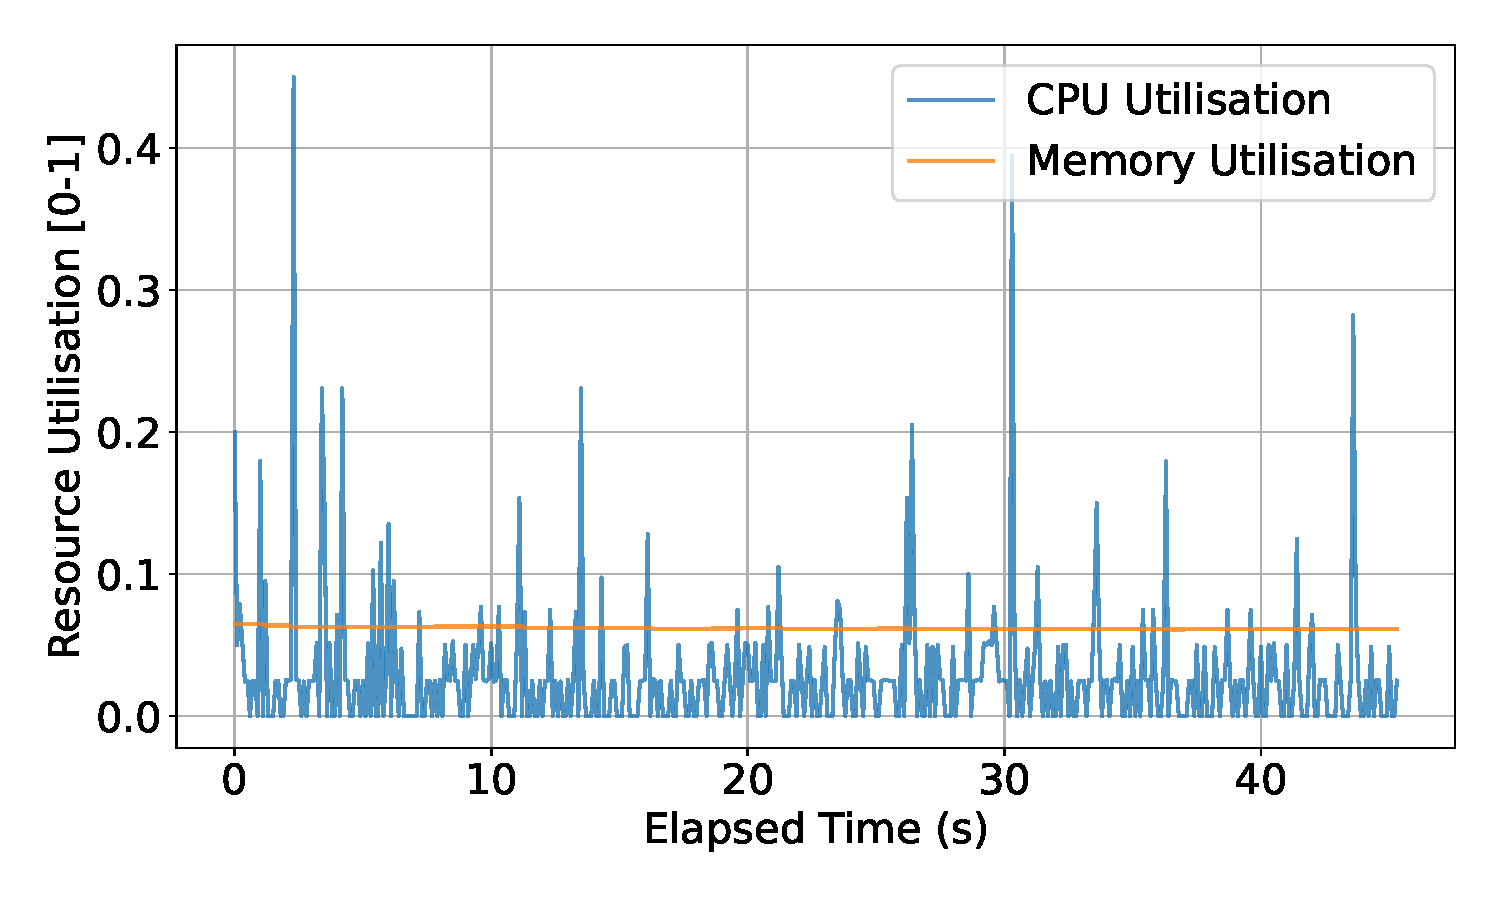
\includegraphics[width=0.45\textwidth]{images/utilisation-baseline.pdf}
    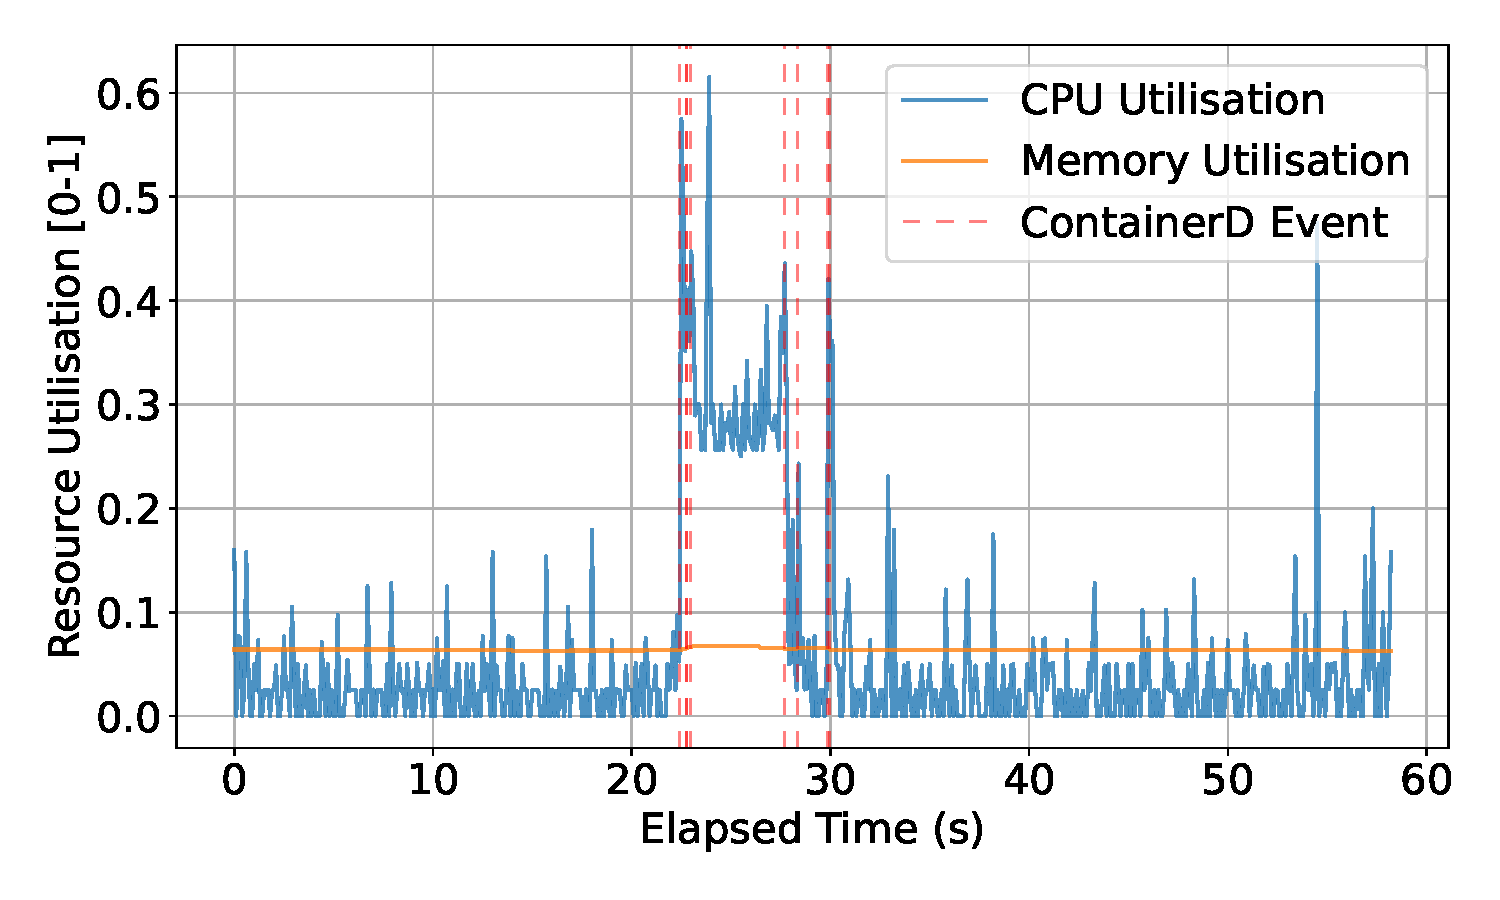
\includegraphics[width=0.45\textwidth]{images/utilisation-single.pdf} \\
    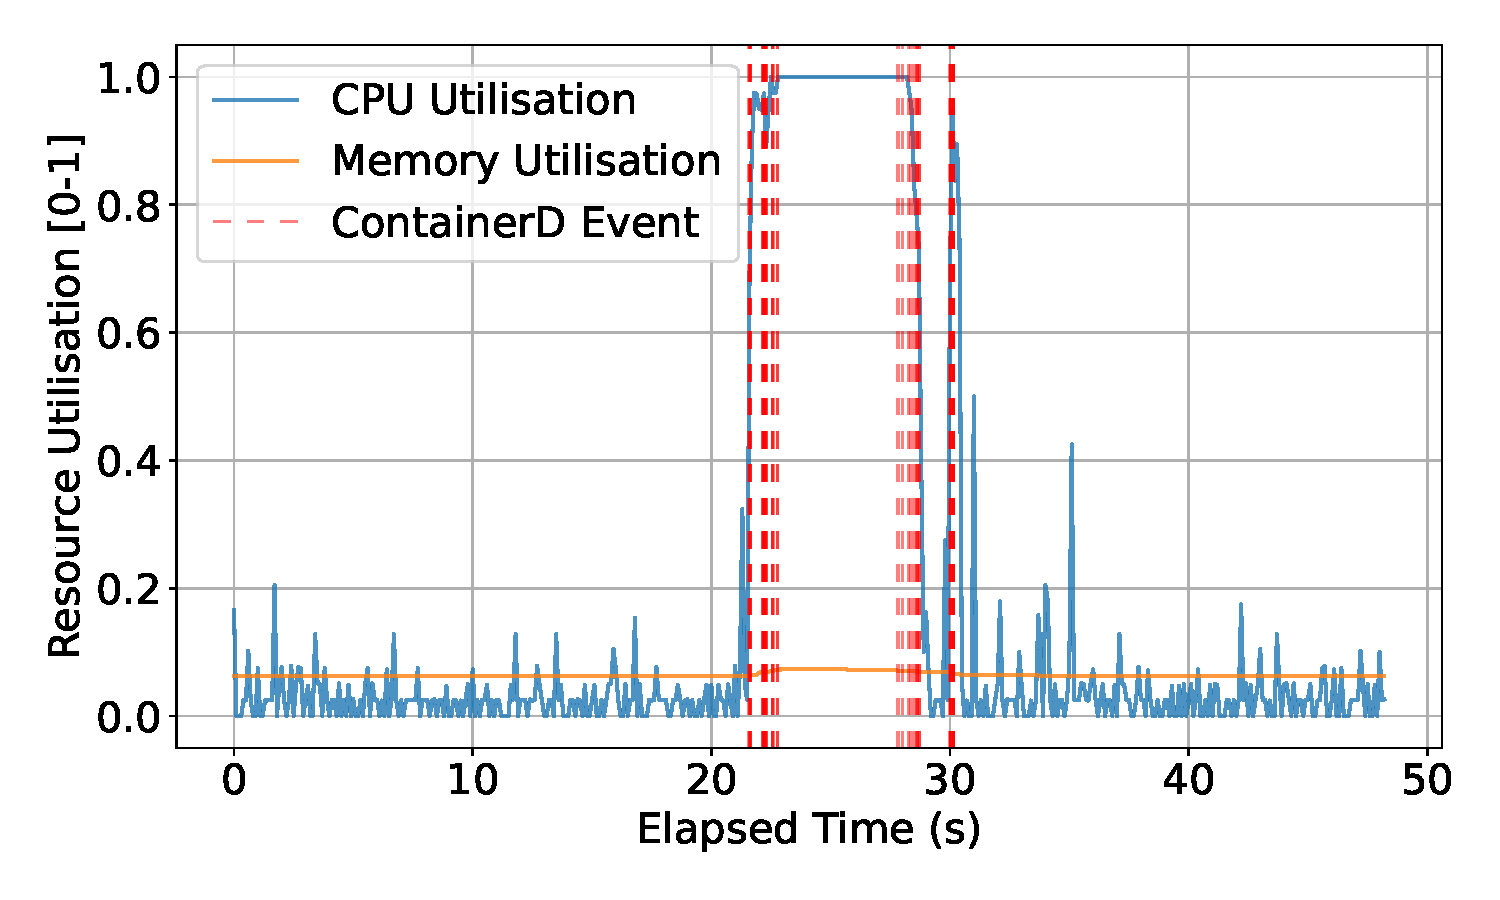
\includegraphics[width=0.45\textwidth]{images/utilisation-smallbatch.pdf}
    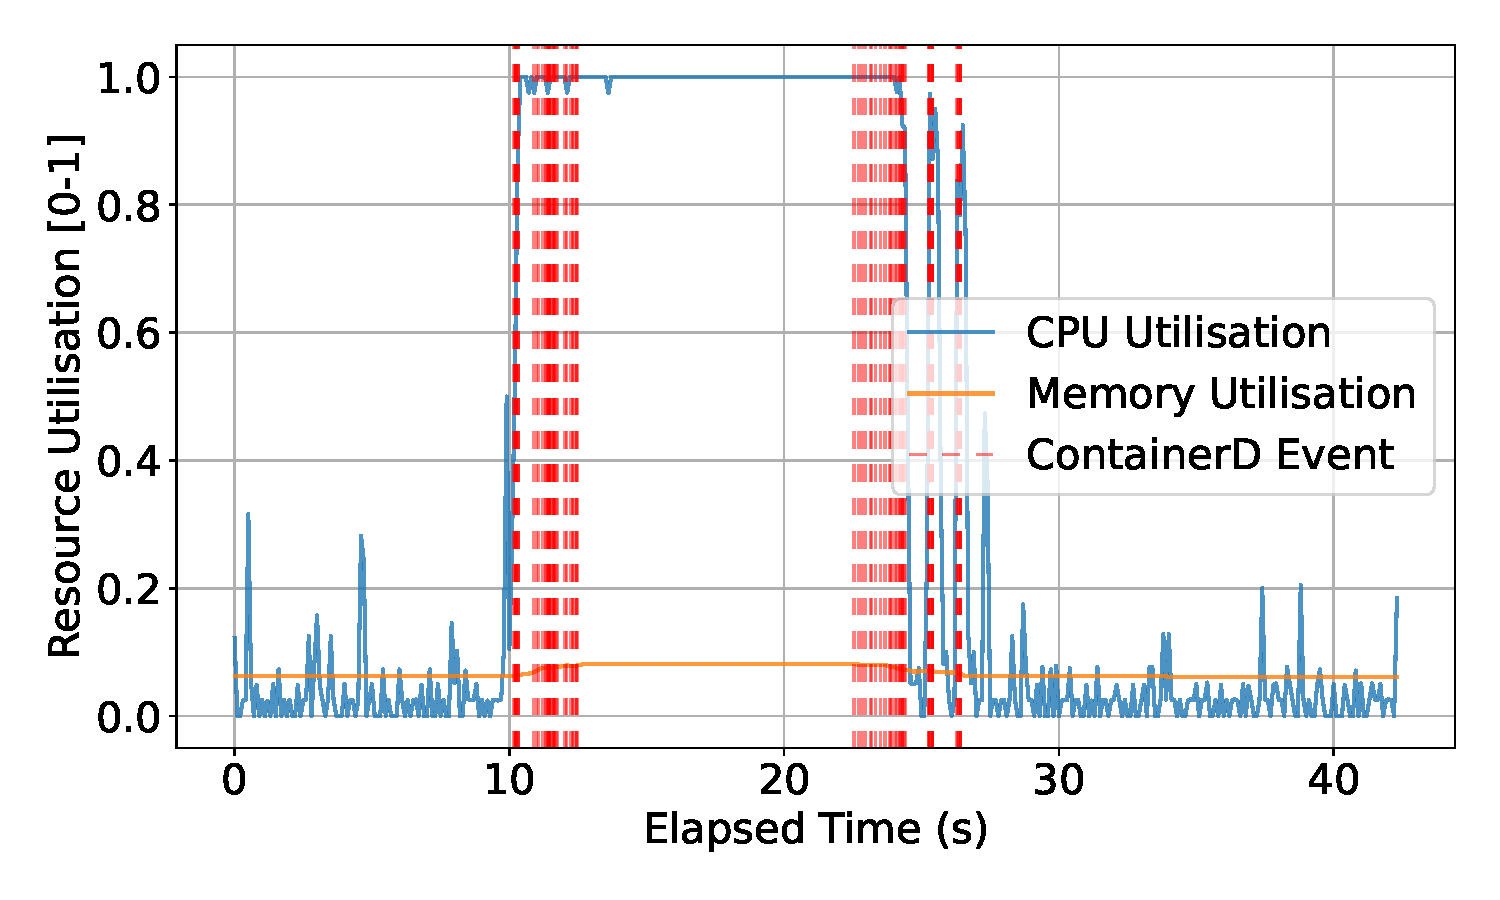
\includegraphics[width=0.45\textwidth]{images/utilisation-bigbatch.pdf}
    \caption{In this figure we sample CPU and memory utilisation from
    values of \texttt{/proc/stat}, \texttt{/proc/meminfo} at 10Hz during various
    Kubernetes workloads.}
    \label{fig:utilisation-eval}
\end{figure}

Figure \ref{fig:utilisation-eval} demonstrates how the [0,1]-normalised
metrics can quickly respond to the resource usage workloads of different sizes.

\subsubsection{Issues of using CPU Utilisation}
\label{sec:issue-with-util}
Early prototypes using only utilisation metrics showed poor throughput compared
to the default \verb|kube-scheduler|. When Pods requested
100 milliCPU the \verb|kube-scheduler|, Nodes would have $\approx$ 45
Pods running on them at once. In contrast, \textsc{Carico}, using only utilisation
telemetry, would allocate at most 5 Pods concurrently per Node. Although both
approaches achieved 100\% CPU utilisation, \verb|kube-scheduler| achieved a
short Job Completion time while having a long-tailed distribution of individual
Pod Completion times.

\begin{figure}[H]
    \centering
    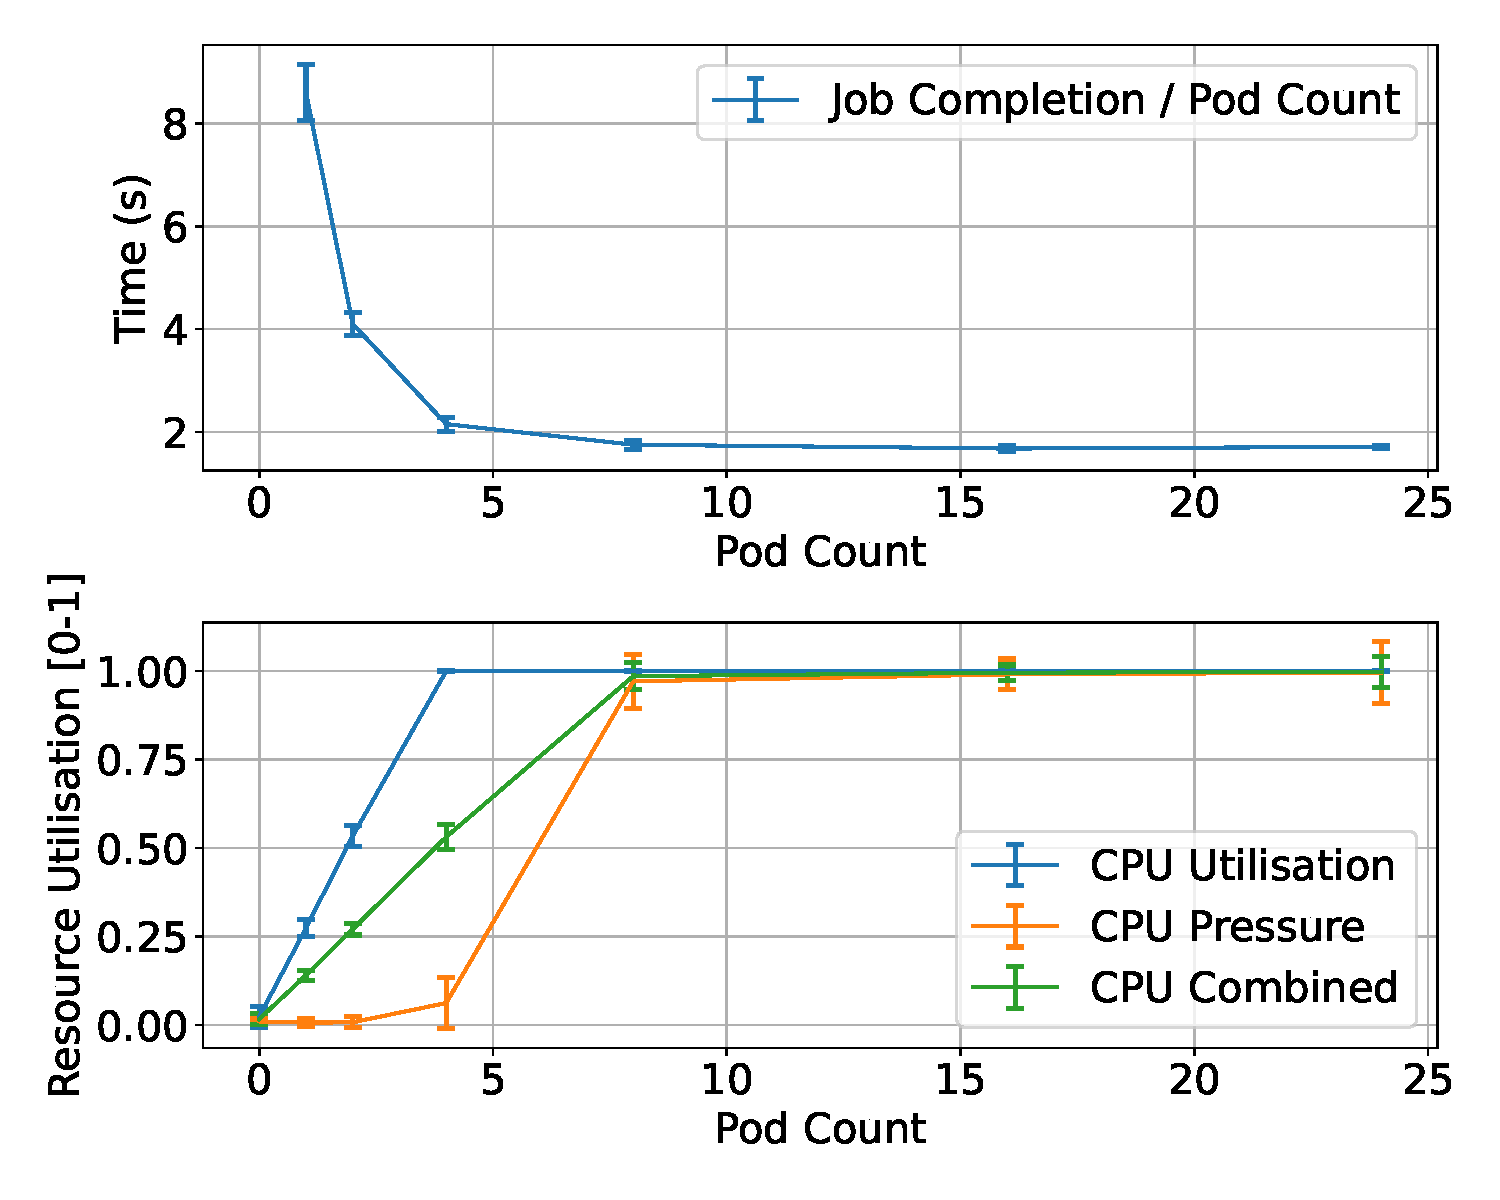
\includegraphics[width=0.45\textwidth]{images/podcount-util-pressure.pdf}
    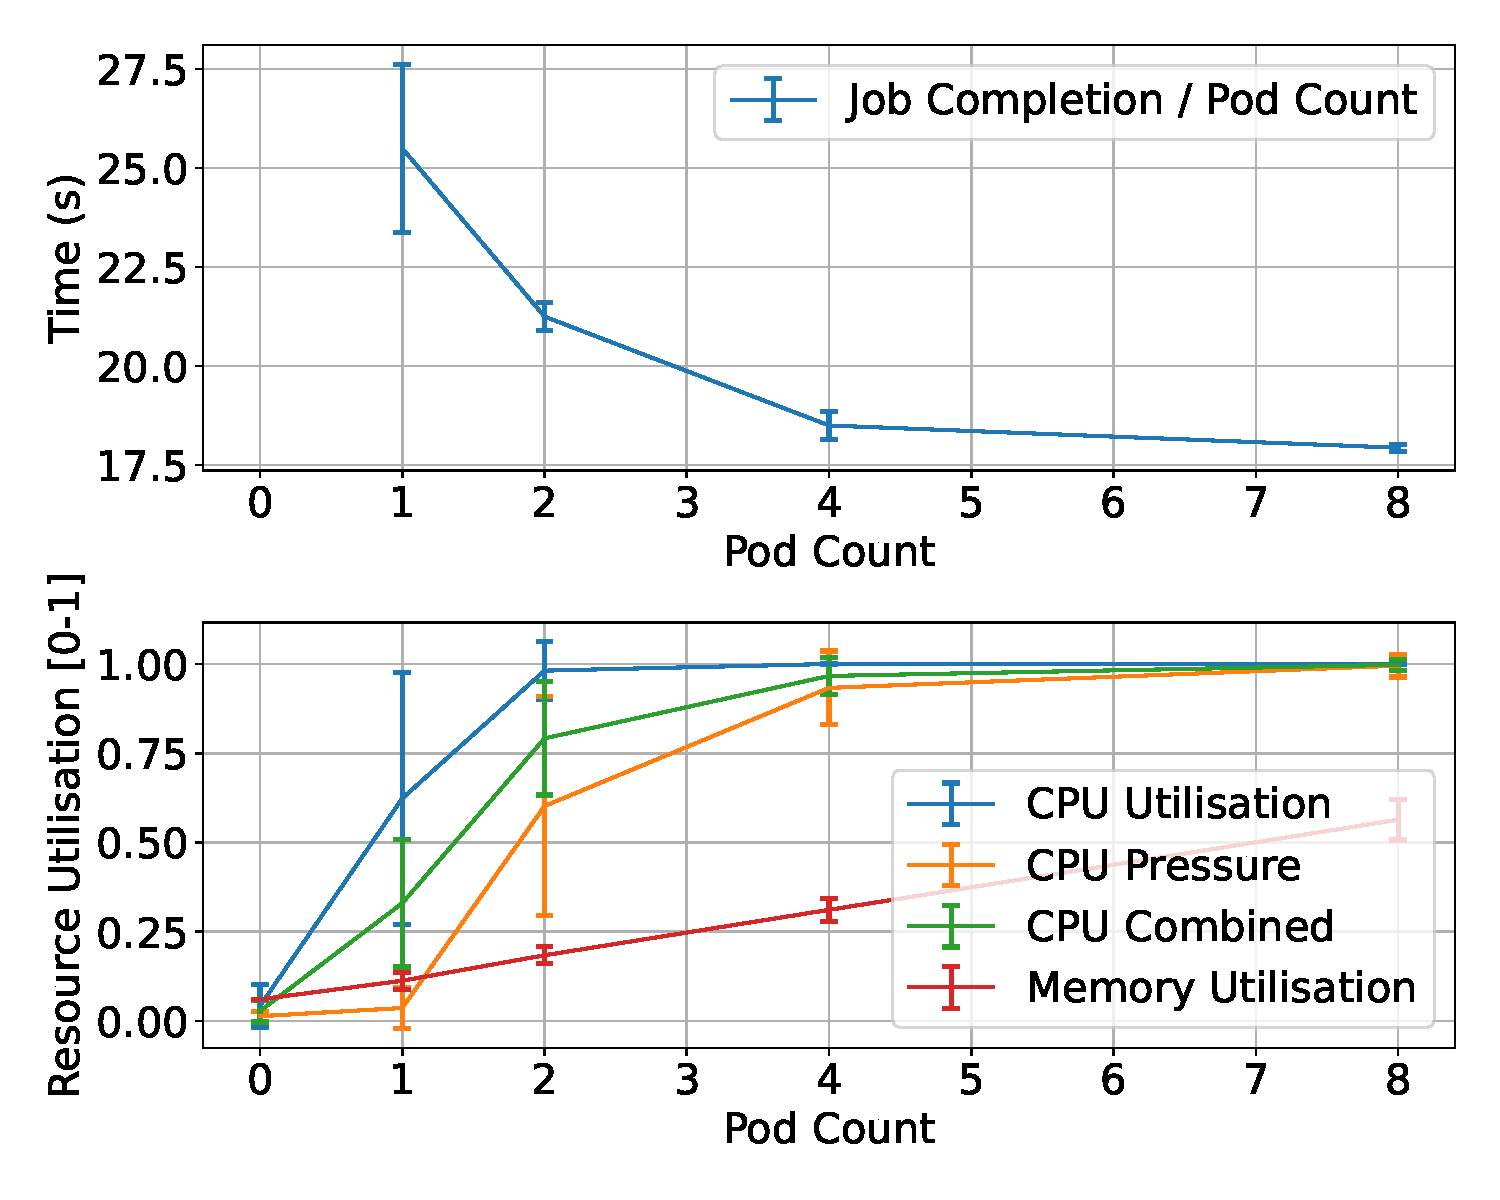
\includegraphics[width=0.45\textwidth]{images/ml-podcount-util-pressure.pdf}
    \caption{Collected resource metrics during various Kubernetes workload.}
    \label{fig:podcount-util-pressure}
\end{figure}

Further investigations, shown in Figure \ref{fig:podcount-util-pressure},
revealed that even after a Node achieves 100\% CPU utilisation, the contribution
of each Pod to the Job Completion time decreases: running more Pods on a Node
resulted in higher throughput. As the cluster runs on virtual machines (VMs), I
hypothesise that the hypervisor inadvertantly masks contention effects like
cache and CPU thrashing when providing a hardware abstraction. Consequently,
high CPU utilisation does not correlate with performance degradation, and thus,
is not an accurate measure of capacity.

\subsubsection{Combining CPU Utilisation and CPU Pressure}
[0,1]-normalised \verb|/proc/pressure| total metrics,
\[ \text{CPU Pressure} = \Delta \text{total} \times \text{polling frequency} \]
aren't sufficient as they do not initially exhibit a linear relation with Pod
count (Figure \ref{fig:podcount-util-pressure}). This would lead to
unreasonably low intial Per-Pod-Cost estimations and an inflated advertised Node
Pod-Capacity. However, by combining CPU utilisation and CPU pressure,
\[ CPU = \frac{\text{CPU Utilisation} + \text{CPU Pressure}}{2} \]
the resulting metric exhibits a pseudo-linear relation with Pod count and
doesn't saturate to quickly (Figure \ref{fig:podcount-util-pressure}): it ouputs
1 when \verb|/proc/pressure| indicates persistant CPU demand (at least one
thread always waiting)

\subsection{Filtering Metrics}
While \textsc{Carico} does not perform peak detection, its Capacity signal is
still susceptible to short-lived spikes. As previously noted,  Pod creation and
deletion incur visible resource usage spikes. These spikes introduce noise into
both the Node's local model and its Capacity signal. As a noisy signal
would result in inaccurate baseline Capacity and Per-Pod-Cost estimation, a
low-overhead signal filter was required.

Dynamic Exponential Moving Average (EMA) automatically adjusts its smoothing
factor $\alpha$, and thus its responsiveness, based on predefined conditions.
As first-hand investigations showed that container events resource spikes last
$\approx$200 milliseconds, Dynamic EMA can be used to
suppress container-event caused spikes (typically $\approx$ 200ms) using a small
$\alpha_{\text{slow}}$, while sustained changes (spikes $>$ 300ms) causes it to
switch to a larger $\alpha_{\text{fast}}$ for rapid convergence.
\begin{figure}[H]
    \centering
    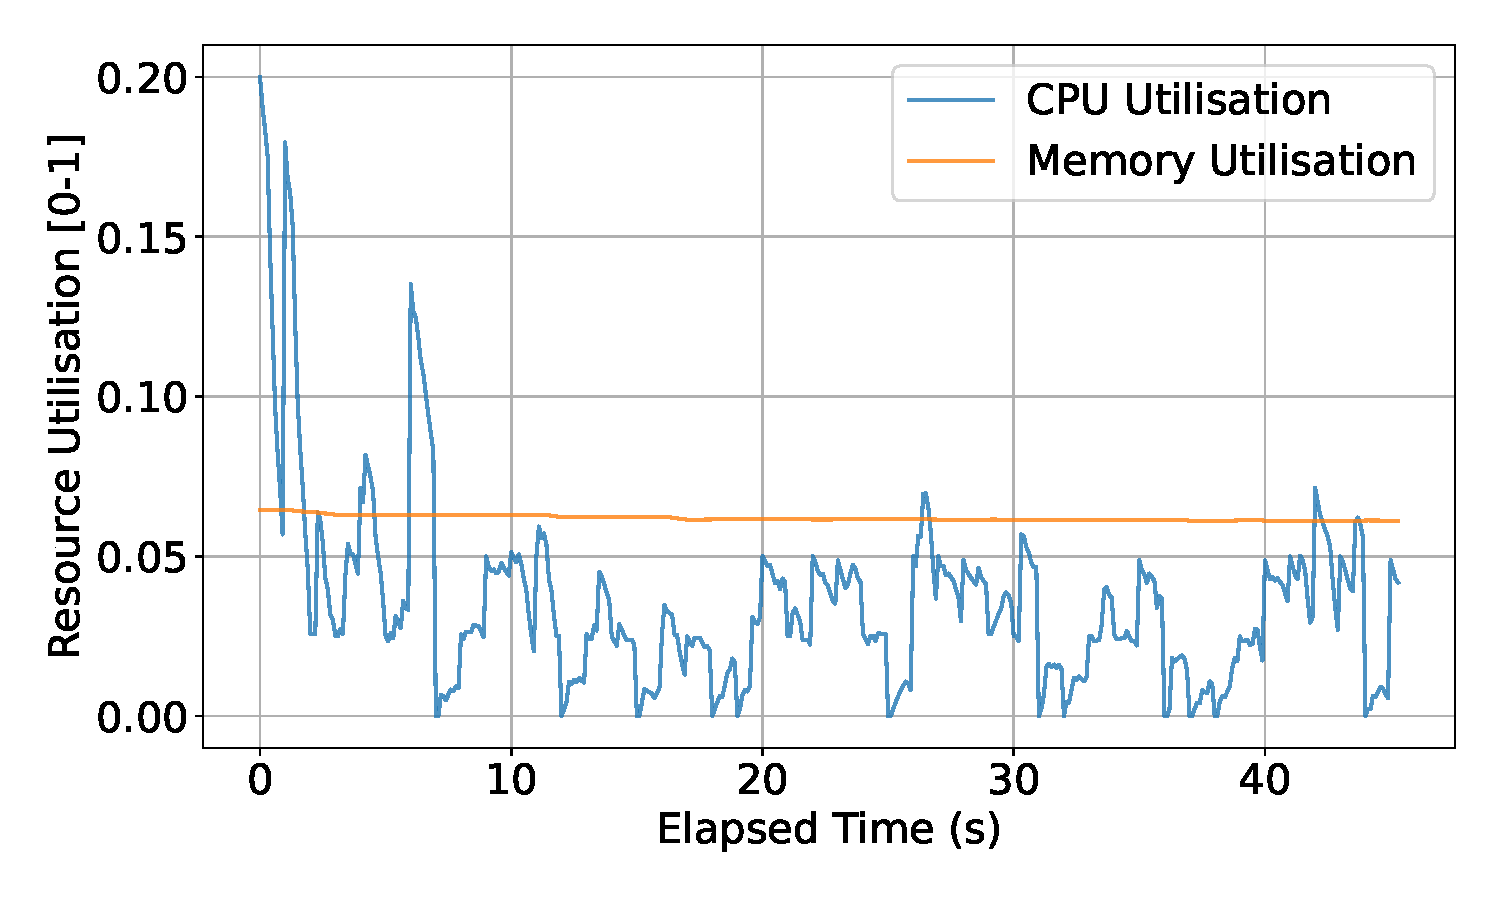
\includegraphics[width=0.45\textwidth]{images/filter-utilisation-baseline.pdf}
    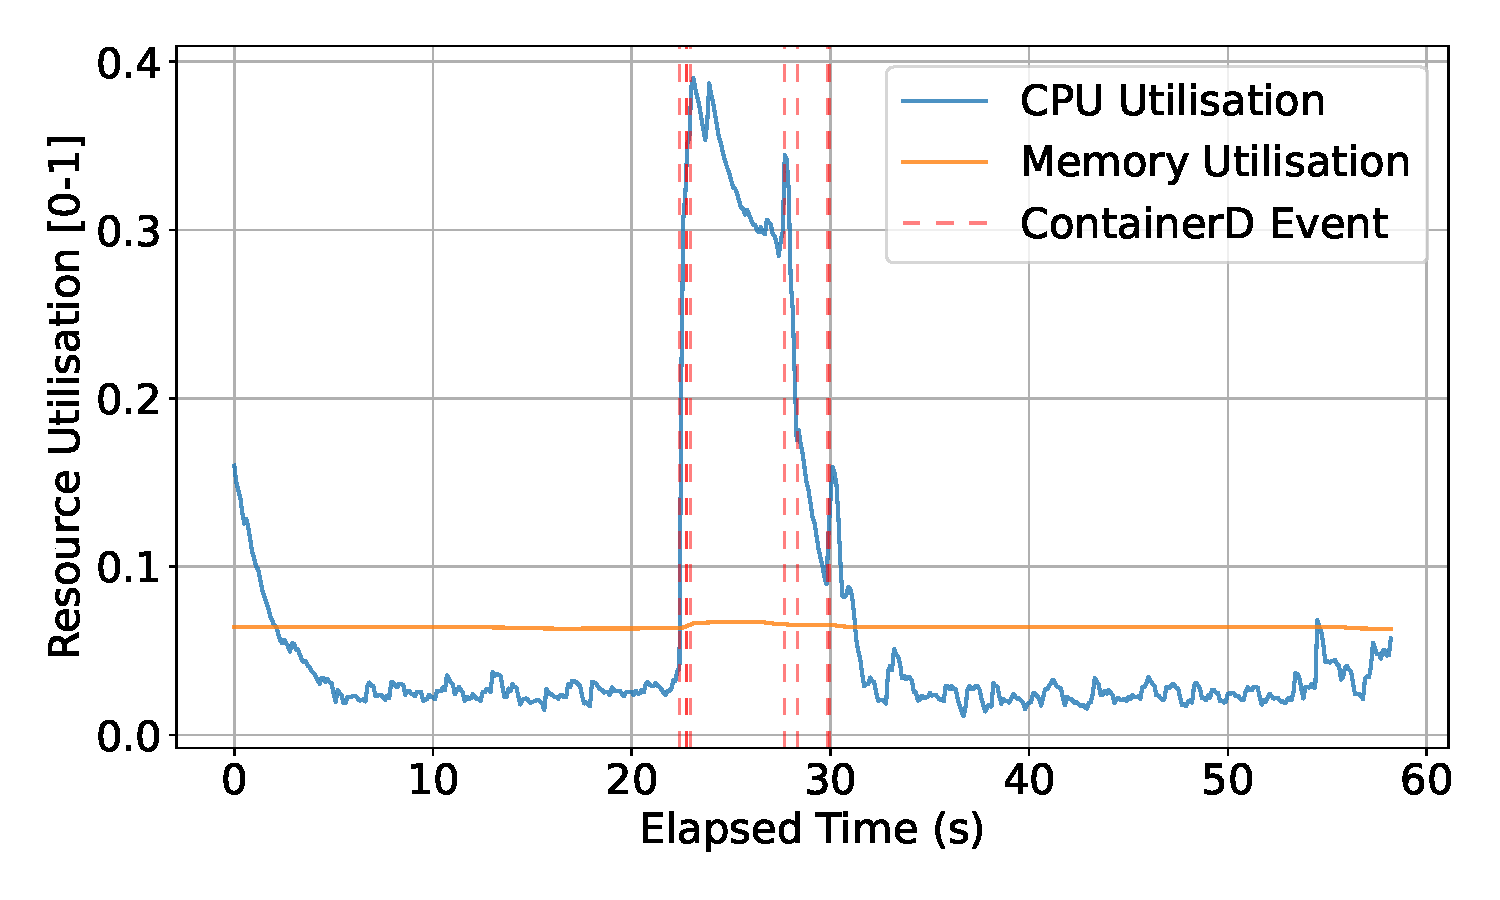
\includegraphics[width=0.45\textwidth]{images/filter-utilisation-single.pdf} \\
    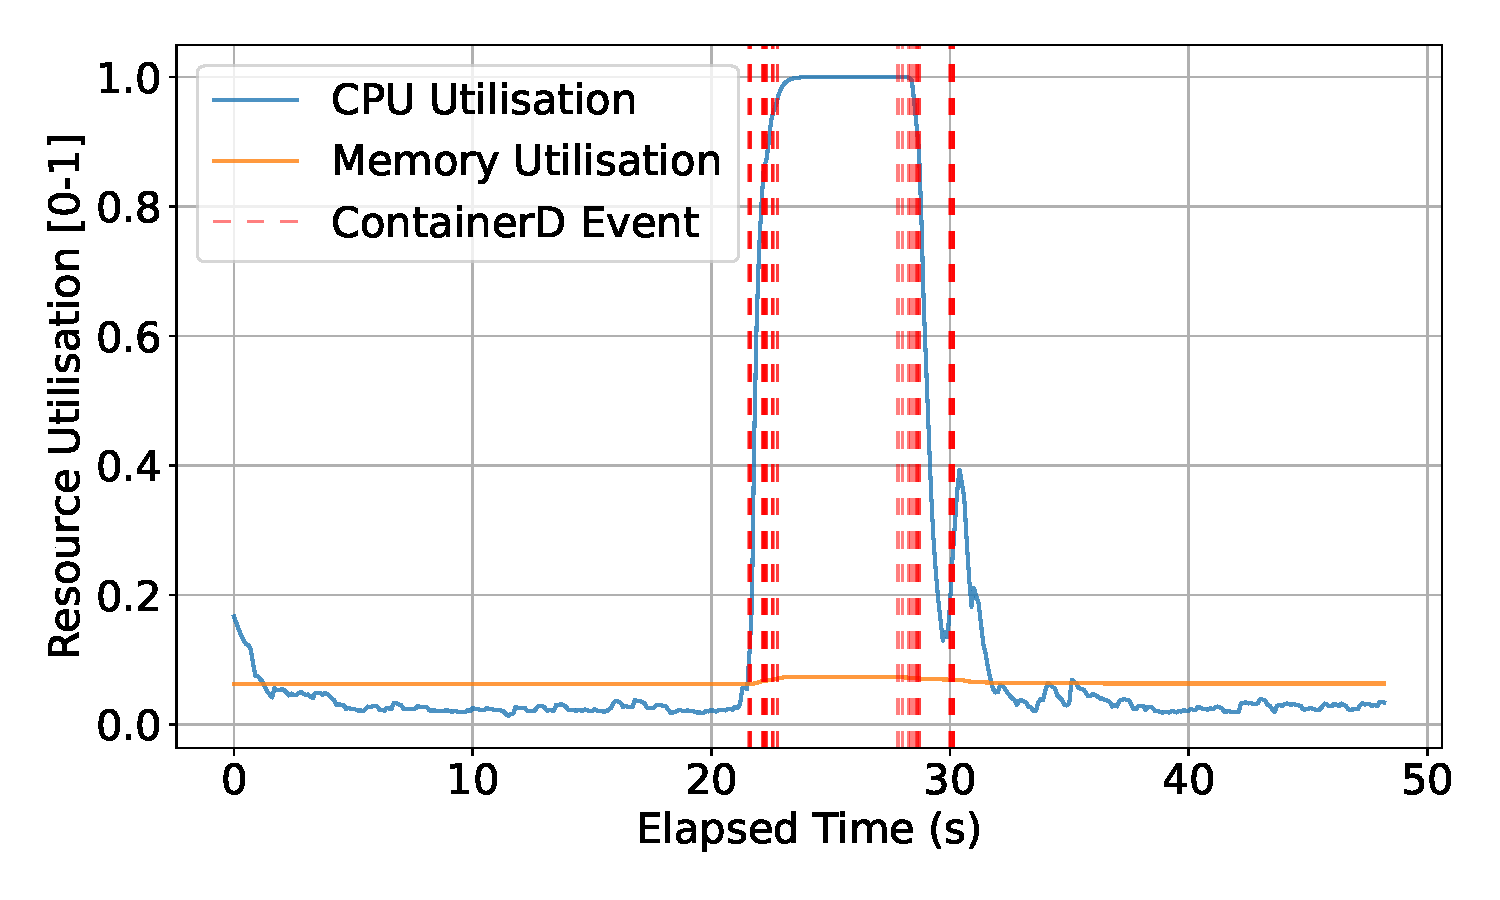
\includegraphics[width=0.45\textwidth]{images/filter-utilisation-smallbatch.pdf}
    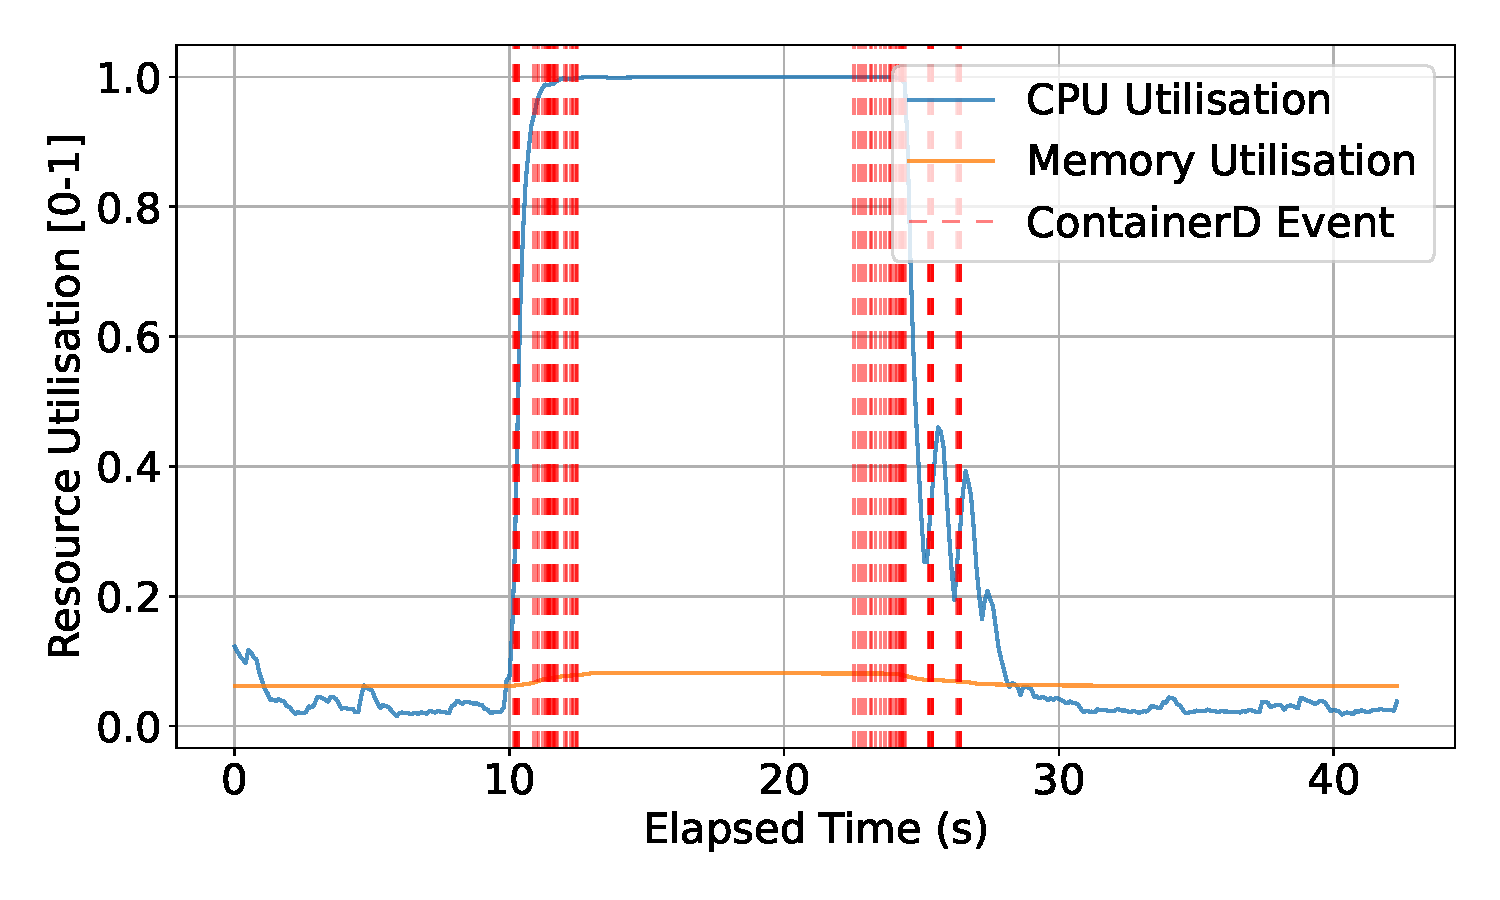
\includegraphics[width=0.45\textwidth]{images/filter-utilisation-bigbatch.pdf}
    \caption{This figure shows the smoothed metrics under different workloads.}
    \label{fig:filtered-metrics-eval}
\end{figure}

Comparing Figure \ref{fig:utilisation-eval} and Figure
\ref{fig:filtered-metrics-eval} reveals the impact of Dynamic EMA on the
collected telemetry.

% Filtering the signal directly, rather than the telemetry, was considered but
% rejected as it would still allow container-event resource spikes to pollute the
% local model.
%
\subsection{Signal Generation}
% The \textsc{Carico} Pod calculates its Capacity signal at 1Hz. This matches the local
% model update frequency, ensuring that the Capacity signal tracks with the local
% model. While a higher frequency would provide the central scheduler a more
% current view of a Node's resource status, it would also increase resource
% overhead. This overhead would reduce the available resources to other
% Pods and could also lower the baseline Capacity signal, potentially reducing
% the capacity a Node advertises.
%
To verify Capacity signal's implementation, I test a \textsc{Carico} Pods under
the scenarios described in Section \ref{sec:signal-example-scenario}.

\begin{figure}[ht]
    \centering
    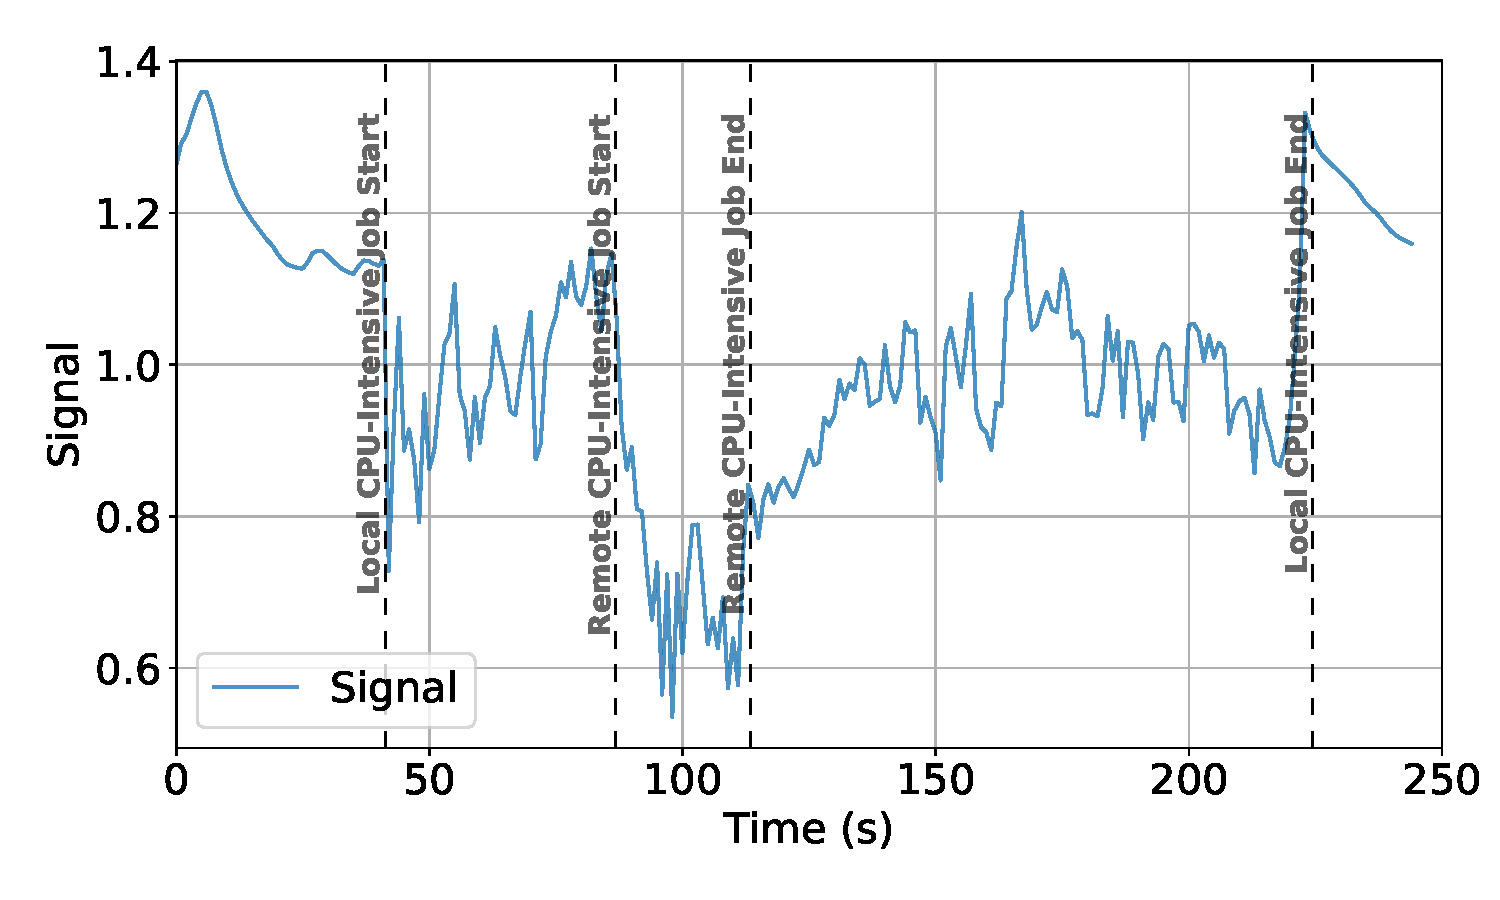
\includegraphics[width=\textwidth]{images/signal-with-cpu.pdf}
    \caption{The calculated capacity signal of a Node running \texttt{ng-stress
    --cpu=8 --cpu-load=25}. While running this workload, $1000$ Pods running
    \texttt{bpi(2000)} were scheduled across surrounding Nodes.}
    \label{fig:signal-evaluation-cpu}
\end{figure}
%
% Figures \ref{fig:signal-evaluation-cpu} and \ref{fig:signal-evaluation-mem}
% demonstrates how a Node's capacity signal reacts to changes in surrounding
% workloads when experiencing different resource usage. In Figure
% \ref{fig:signal-evaluation-cpu}, the measured Node is running a light
% CPU-focused workload.

Figure \ref{fig:signal-evaluation-cpu} shows the Capacity signal of a Node when
running a light CPU-focused workload (\texttt{ng-stress --cpu=8 --cpu-load=25}),
while the remaining Nodes in the cluster execute a CPU-intense workload
(\texttt{bpi(2000)}). The measured Node's capacity signal drops once the
CPU-intense workload is scheduled on its peers. This is expected as the
subspaces of surrounding Nodes, and thus the aggregated subspace, will reflect a
more costly CPU-focused workload (larger $\sigma_1$).  After aggregating its
subspace, combinings its unchanged resource usage with the new increased
expected workload (reflecting in $\sigma_1 u_1$) results in a smaller $k$ (fewer
units of this workload can be added), and thus a lower Capacity signal.

\begin{figure}[ht]
    \centering
    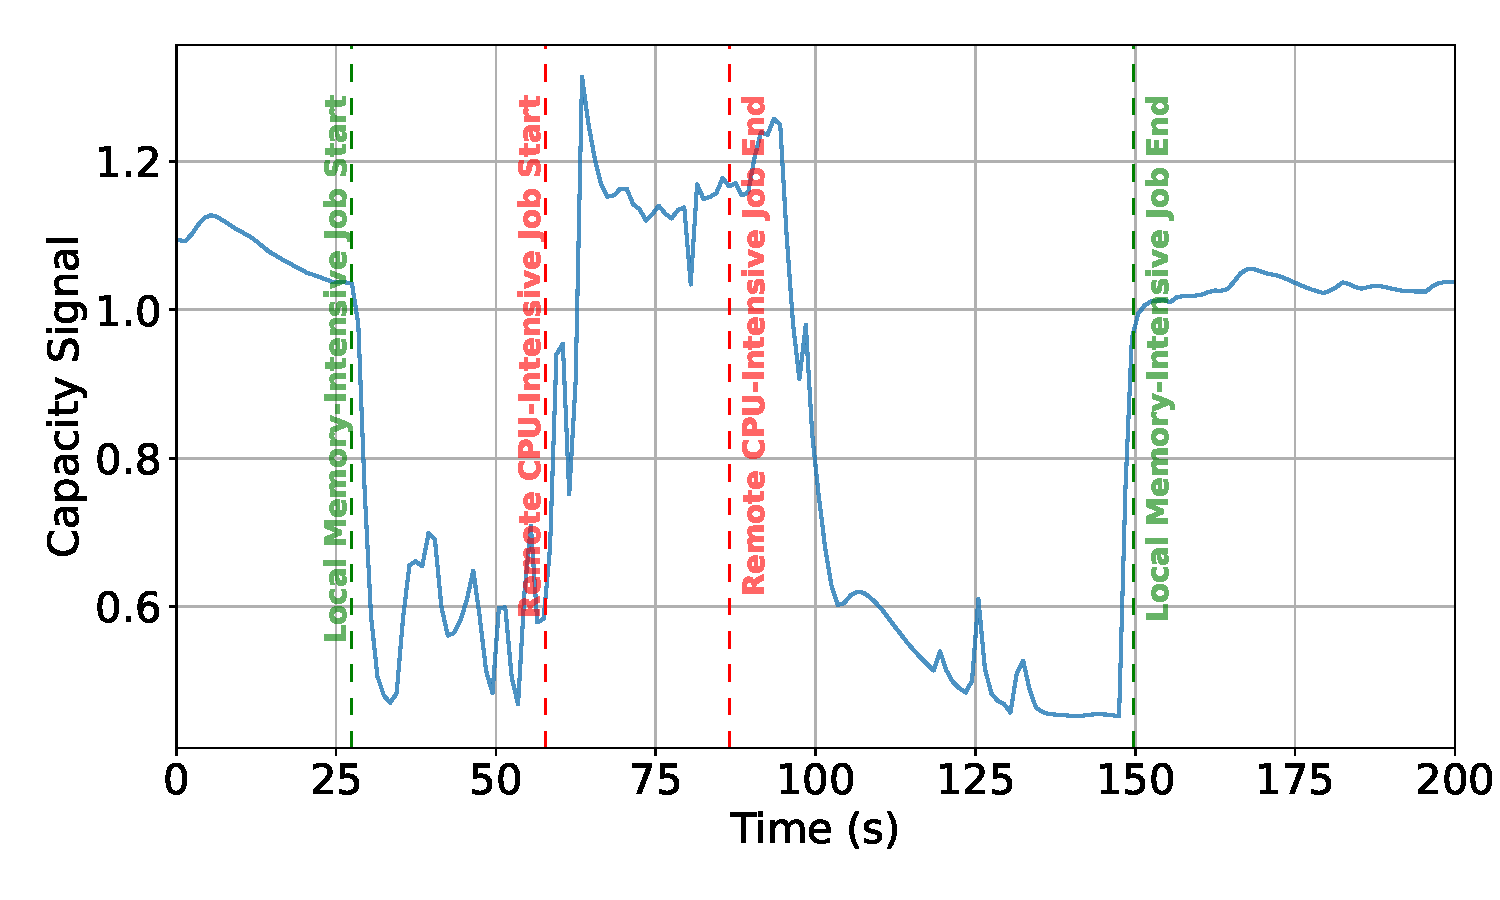
\includegraphics[width=\textwidth]{images/signal-with-memory.pdf}
    \caption{The calculated capacity signal of a Node running \texttt{ng-stress
    --vm=4 --vm-bytes=4G}. While running this workload, $1000$ Pods running
    \texttt{bpi(2000)} was scheduled across surrounding Nodes.}
    \label{fig:signal-evaluation-mem}
\end{figure}

Figure \ref{fig:signal-evaluation-mem} demonstrates the Capacity signal of a
Node when running a light Memory-focused workload (\texttt{ng-stress --vm=4
--vm-bytes=4G}) with the remaining Nodes in the cluster execute the same
CPU-intense workload as in the earlier scenario. Like before, the global
aggregated subspace reflects a heavy CPU-focused workload. However, when the
measured Node combines this new expected workload with its current
memory-focused resource usage, a larger $k$ is required to reach a resource
limit.

We can conclude that the \textsc{Carico} Pods behave correctly.

\subsection{Calculating Cost and Capacity}
To implement a reservation mechanism, \textsc{Carico} assumes the ability to
measure Pod count and estimate the Baseline Capacity Signal and Per-Pod-Cost.
Due to the resource constraints of the \textsc{Carico} Pods, the chosen
estimation technique must be lightweight and operate on a single pass of
telemetry. Furthermore, Kubernetes fast-paced and noisy environment, means the
techniques must handle handle dynamic workloads and noise from container churn.

\subsubsection{Detecting Pod Events}
\label{sec:listeners-comparison}
The quality Capacity signal is crucial to the accuracy of estimations. Dynamic
EMA can't fully eliminate the noise from the container runtime (shown in Figure
\ref{fig:filtered-metrics-eval}). Therefore, some noise will bleed into the
Capacity signal and reduce the accrucy of estimates. To combat this, early
detection of container events can halt estimations during these bursts. Thus,
the requirements for an event listener are:
\begin{itemize}
    \item Detect the creation and deletion of Pods to establish a Pod count
    \item Provide warning for potential container-caused churn
\end{itemize}

\begin{figure}[ht]
    \centering
    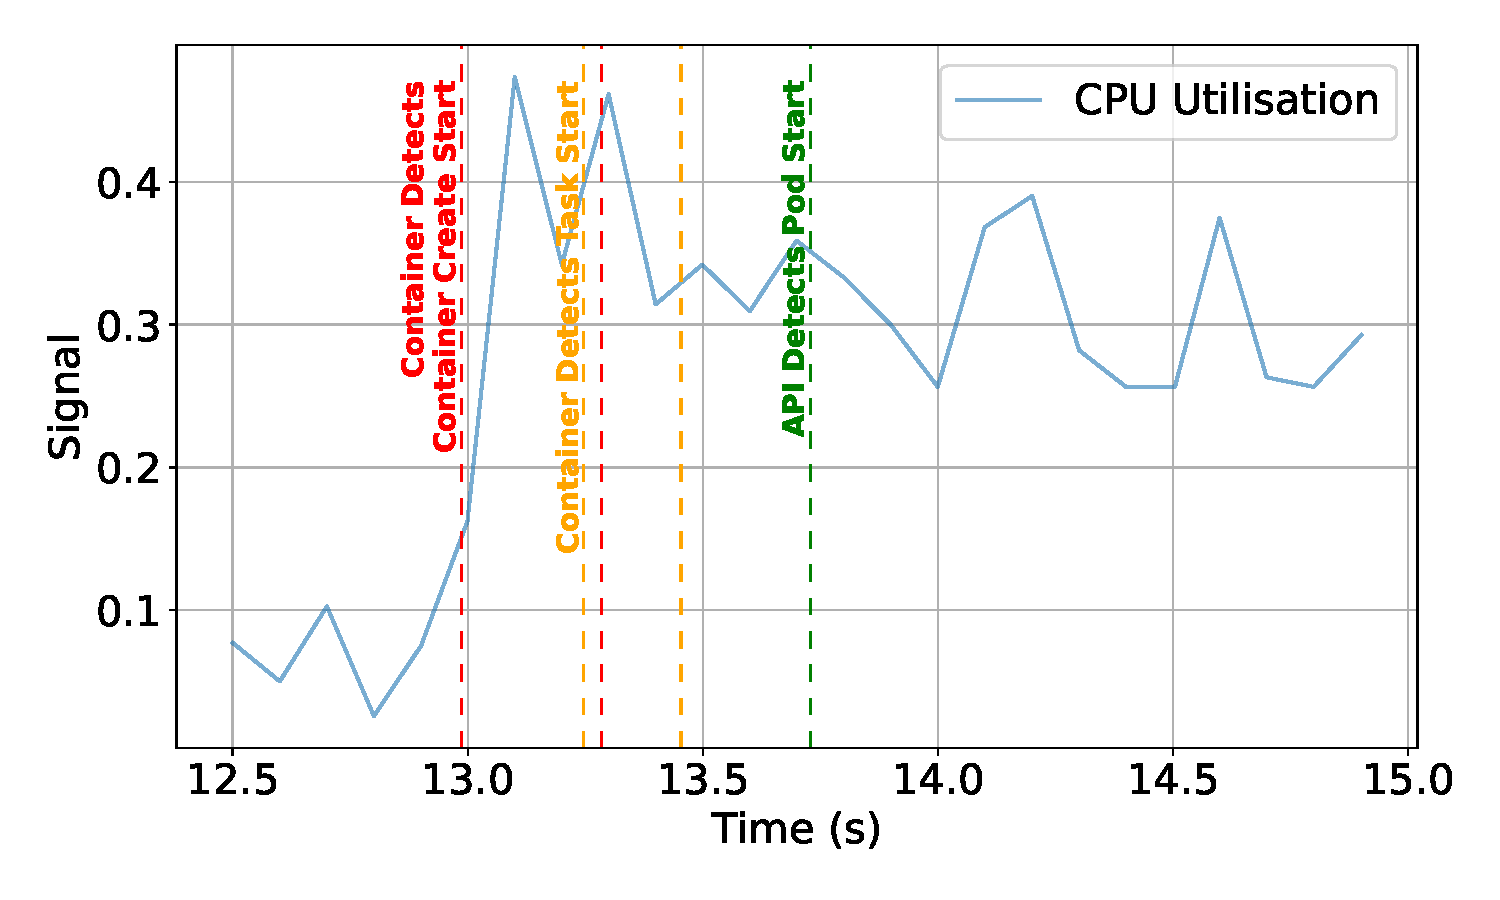
\includegraphics[width=\textwidth]{images/event-comparison-start.pdf}
    \caption{When different event listeners detected the creation of a Pod.}
    \label{fig:event-evaluation-start}
\end{figure}

\begin{figure}[ht]
    \centering
    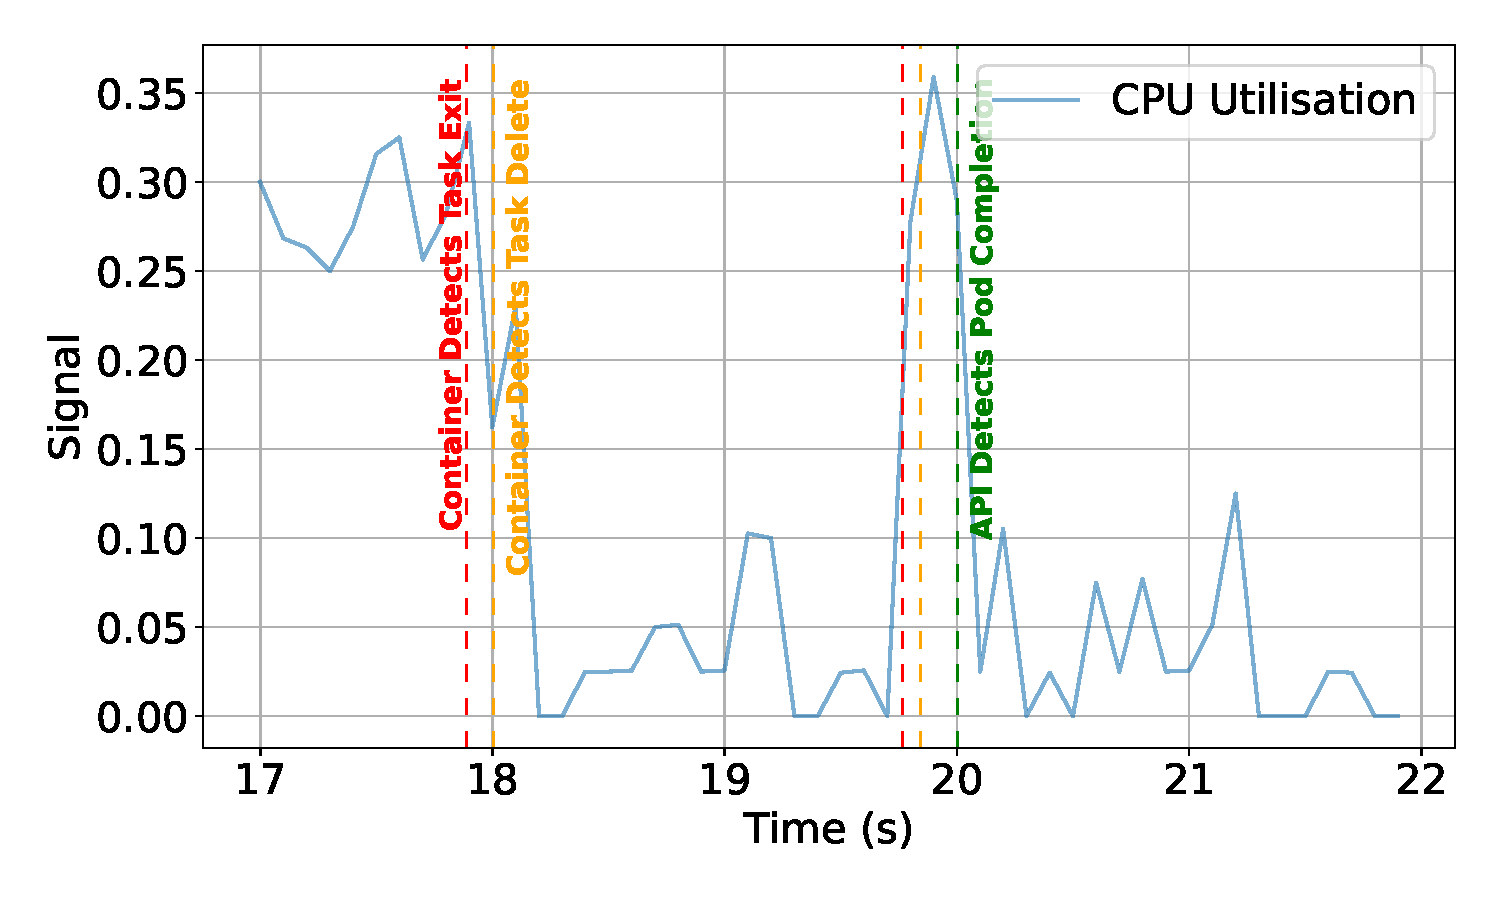
\includegraphics[width=\textwidth]{images/event-comparison-end.pdf}
    \caption{When different event listeners detected the completion of a Pod.}
    \label{fig:event-evaluation-end}
\end{figure}

I investigated two event detection approaches: watching the Kubernetes API vs
ContainerD events. Figures \ref{fig:event-evaluation-start} and
\ref{fig:event-evaluation-end} show that communication latency from the
Kubernetes API causes its listener to miss container runtime resource spikes,
while initial container events precede the spikes. Though more complex, handling
ContainerD events directly provides sufficient warning for container churn.

\subsubsection{Estimating Pod-Cost}
\label{sec:estimating-cost}
A Kalman filter \cite{} is a powerful lightweight streaming algorithm used for
estimating the true state of a dynamic from a series of noisy and uncertain
measurements. It's widely applied in fields like navigation (GPS), robotics,
signal processing and control systems. Its ability to estimate a system's state
from noisy measurements makes it suitable for this dynamic environment.

I devised three Kalman filter-based approaches to estimating reservation costs.
\begin{itemize}
    \item 1D Kalman Filter predicting reservation cost based on the function:
        \[\Delta \text{Capacity signal} = \Delta \text{\# Running Pods} \times
        \text{Per-Pod-Cost}\]
    \item 2D Kalman Filter to predict the signal based on the function:
        \[\text{Capacity signal} = \text{Baseline Capacity signal} - \text{Per-Pod-Cost}
        \times \text{\# Running Pods}\]
    \item Two separate 1D Kalman Filters predicting the equation:
        \[\text{Capacity signal} = \text{Baseline Capacity signal} -
        \text{Per-Pod-Cost} \times \text{\# Running Pods}\]
        Here, each filter learns a separate variable. This separation prevents
        non-zero covariance entries in the state covariance matrix ($\mathbf{P}$),
        mitigating oscillations observed with a single 2D Kalman filter.
\end{itemize}
To ensure accurate estimates, estimations are halted whenever the Capacity signal
reaches zero. When this occurs, it indicates that at least one resource is fully
utilised, and additional Pod won't further decrease the observed Capacity
signal. Filters may account for this behaviour by inaccurately decrease the
Per-Pod-Cost, leading to an inflated advertised Pod-Capacity.

\begin{figure}[H]
    \centering
    % 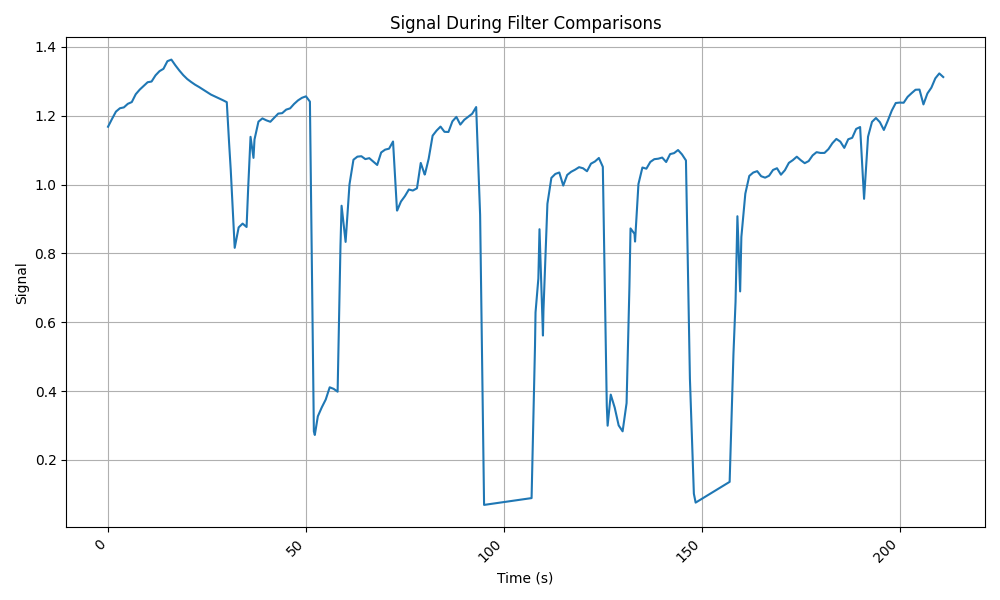
\includegraphics[width=0.45\textwidth]{images/filter-signal.png}
    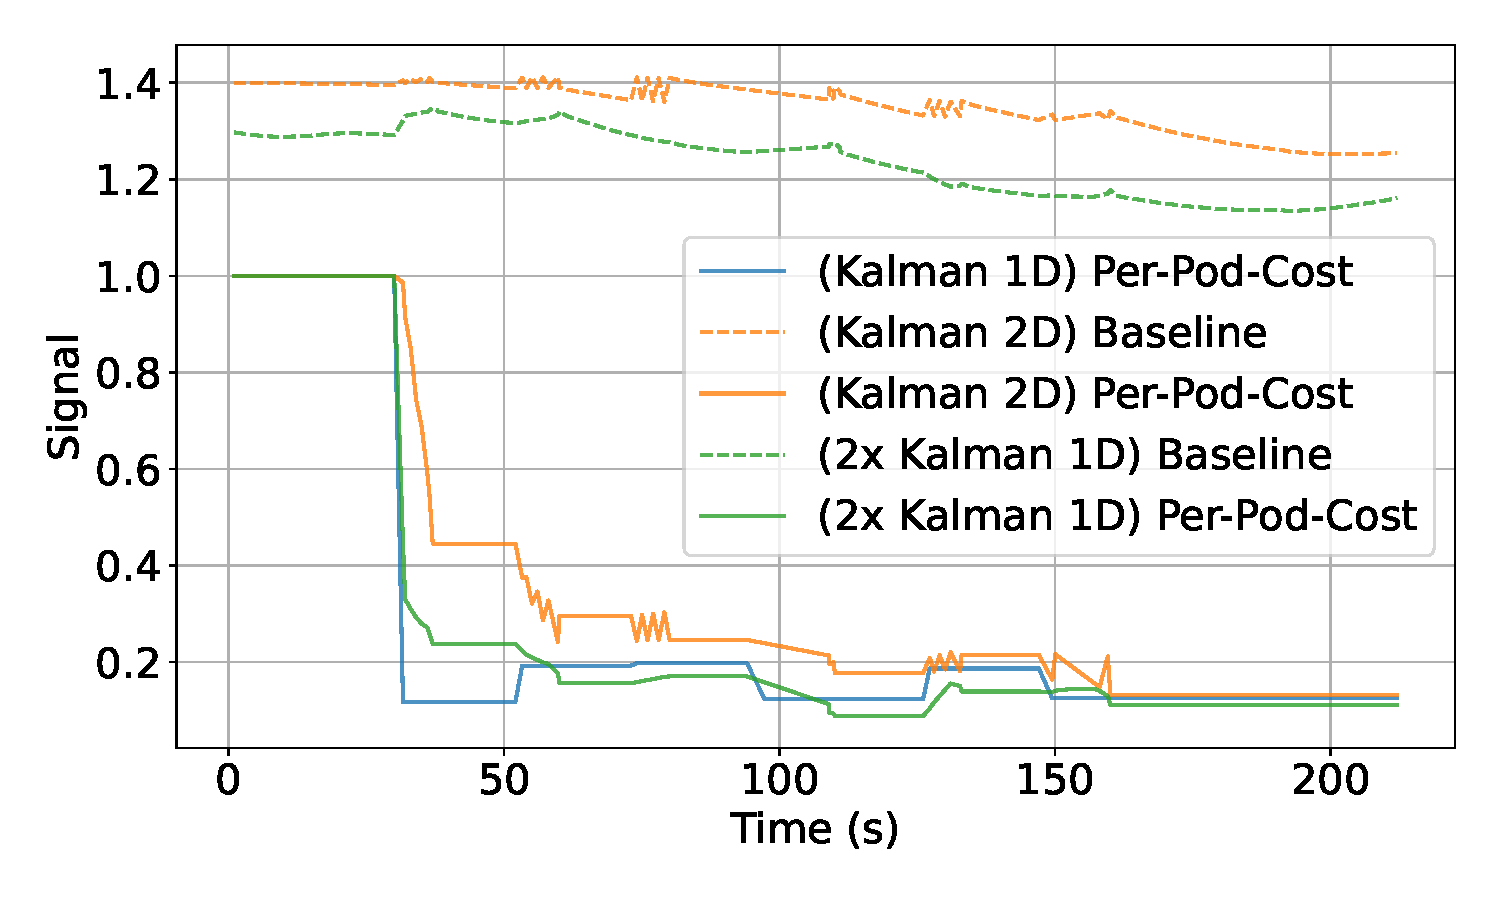
\includegraphics[width=\textwidth]{images/filter-comparison.pdf}
    \caption{The estimates of the Kalman filters when Node experiences
    variable-sized bursts of \texttt{bpi(2000)} Pods.}
    \label{fig:filter-evaluation}
\end{figure}

To identify the optimal approach, I observed each methods' when under the same
workloads (shown in Figure \ref{fig:filter-evaluation}). The $\Delta$-based
Kalman filter accurately estimated Per-Pod-Cost, but being one-dimensional,
could not estimate the Node's baseline Capacity signal. The 2D Kalman filter
approach provides a simple method for estimating both the Node's capacity and
its per-Pod cost. Faster convergence for the 2D filter was attempted using large
process noise covariance ($\mathbf{Q}$) values. This, however, led to large
oscillations, as the filter adjusted both baseline capacity and cost variables
to correct errors. The dual 1D Kalman filter was inspired by the stability of
the 1D Kalman filter. This filter converged quickly and accurately without
exhibiting the oscillations that plagued the 2D Kalman filter. Therefore, this
final approach was used in the \textsc{Carico} Pod implementation.

\section{Aggregation Server}
\textsc{Pronto} aggregation resembles the distributed agglomerative summary
model (DASM) \cite{}. Local models are aggregated in a "bottom-up" approach
following a tree-structure depicted in Figure \ref{pronto-agg}. While this
approach reportedly requires minimal synchonisation, it demands
multiple dedicated Pods, and Kubernetes' inherent communication latency could
significantly delay global model updates after workload changes.

Therefore, I opted for a ``flat" on-the-fly aggregation approach: when the
Aggregation Server receives an aggregation request with a Node's local model,
instead of aggregating the local model and returning the new global model, the
server first enqueues the local model to be aggregated and returns its current
view of the global model. This implementation trades consistency for latency.

\begin{figure}[ht]
    \centering
    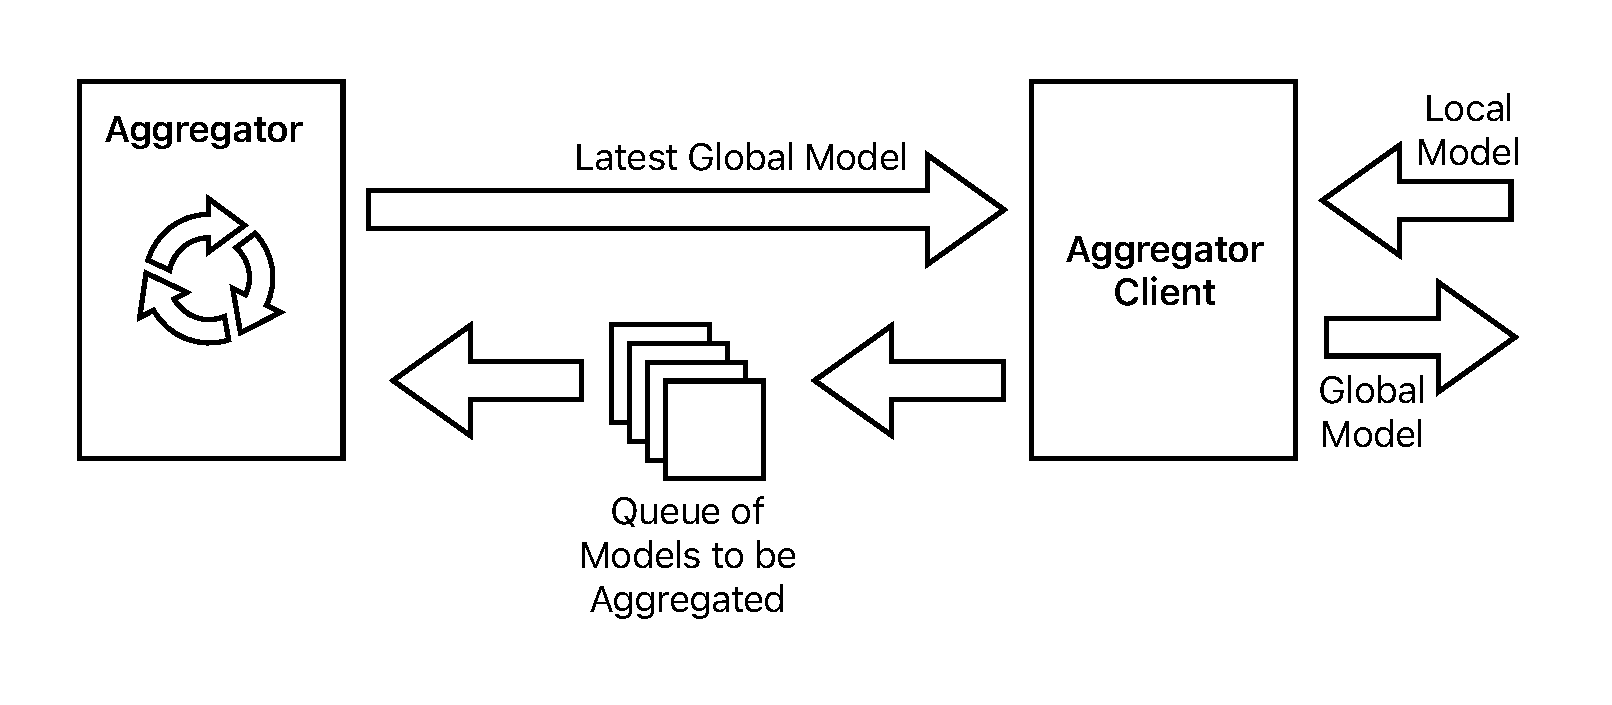
\includegraphics[width=\textwidth]{images/spazio-agg.pdf}
    \caption{The components within the Aggregator Server.}
    \label{spazio-agg-components}
\end{figure}

The Aggregation Server executes a thread which waits on a queue of local models
to aggregate. When the queue is non-empty, the thread pops the local model and
performs a Subspace Merge operation (as defined in \ref{sec:local-merge}). To
balance the influence of each local model, weights $\gamma_{\mathbf{A}} =
\text{\# of Nodes} - 1$ and $\gamma_{\mathbf{B}} = 1$ are used in the
Subspace-Merge (as per Section \ref{sec:local-merge}).
Aggregation clients perform a gRPC call to the address specified by the
Aggregation Service. This gRPC function is implemented by the server and takes
the local model of a Node as its argument. The function first enqueues the local
model to be merged and returns the latest view of the global model. Clients
then aggregate their own local model with the received global model. Decoupling
model aggregation from the gRPC call's critical path reduces server load,
improving its capacity to handle more clients.

\section{Scheduler Pod}
\subsection{Kubernetes Scheduler Plugin}
\begin{figure}[H]
    \centering
    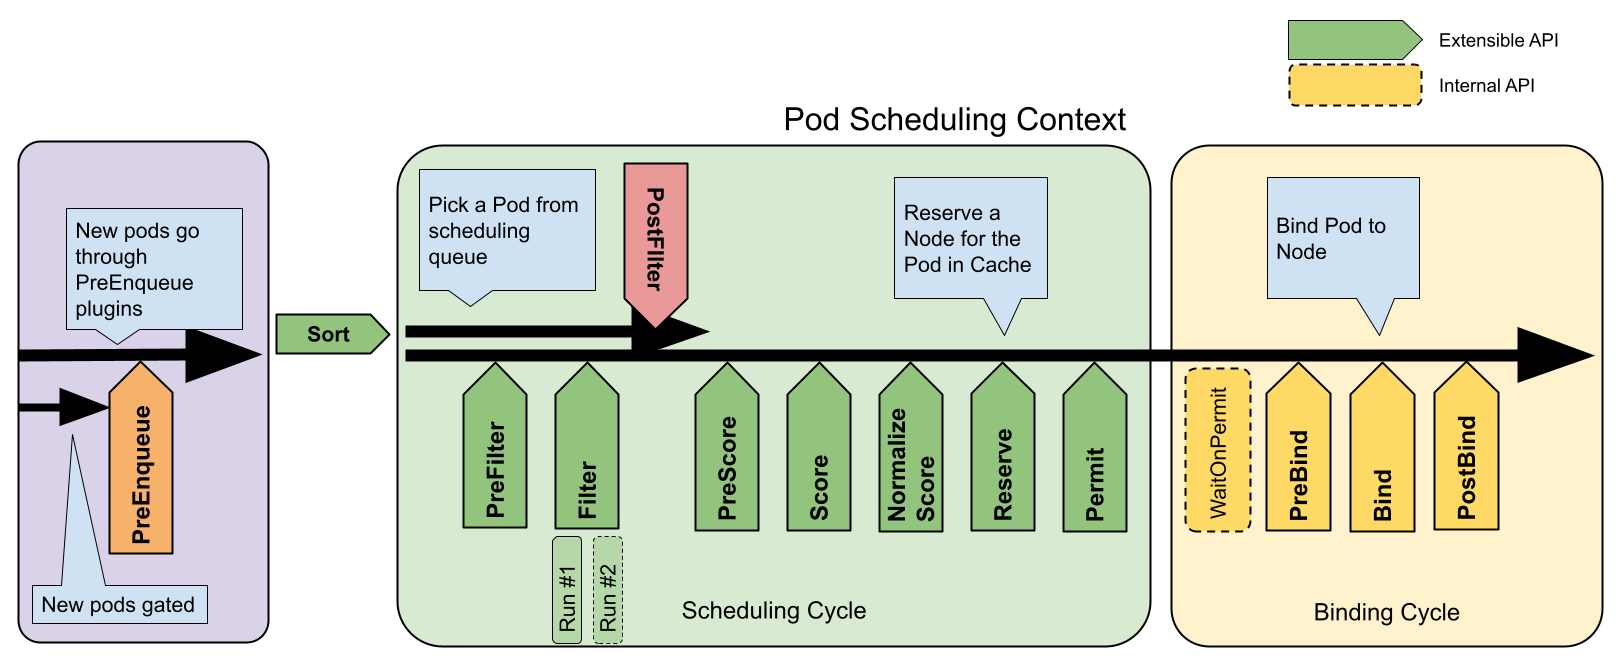
\includegraphics[width=\textwidth]{images/scheduling-framework-extensions.png}
    \caption{The available scheduling framework extension points
    \cite{scheduling-framework}.}
    \label{fig:kube-sched-framework}
\end{figure}
The scheduling framework (depicted in Figure \ref{fig:kube-sched-framework}) is
a pluggable architecture for the Kubernetes scheduler. It defines extension
points at which scheduler plugins register to be invoked. A scheduler plugin can
register to multiple extension points, with each extension point defining an
interface: a set of functions the scheduler plugin has to implement.

Developing a \textsc{Carico}-based scheduler plugin, rather than a standalone
scheduelr, simplified implemention and offered many performance benefits. First,
\textsc{Carico}'s scheduling operations (Section \ref{sec:spazio-cost-capacity}
map well to the framework's extension points. Second, the framework provides
access to efficient, pre-existing data structures and algorithms. Finally,
plugins allow customisation through selective enabling/disabling of default
plugins and ordering of custom ones. This means that the \textsc{Carico} plugin
could be used in tandem with other plugins to improve scheduling decisions.

The \textsc{Carico} scheduler tracks Pod reservations using a \verb|map| (Pod ID
to Node ID) and a Kubernetes API Pod Event Listener. During the Reserve phase, the scheduler
increments the target Node's reserve count and records Pod-Node assignment. When
the API listener detects a Pod transitioning from the 'Pending'
status, if the Pod is in its reservation \verb|map|, the scheduler decrements
the corresponding Node's reserved count.
